\documentclass[a4paper,11pt]{report}

\usepackage{fullpage}
\usepackage{graphicx}
\usepackage{amsmath,amssymb}

\usepackage{bussproofs}
\usepackage{mathpartir}
\usepackage{prooftrees}
\usepackage{color}

\newcommand*\circled[1]{\tikz[baseline=(char.base)]{
    \node[shape=circle,draw,inner sep=2pt] (char) {#1};}}

\usepackage[cache=false]{minted}

\newminted{smalltalk}{
  frame=single,
  framesep=6pt,
  breaklines=true,
  fontsize=\scriptsize,
  linenos
}

\date{\today}

\setlength{\parindent}{0pt}
\setlength{\parskip}{2.5pt}

\begin{document}

\begin{center}
\Large{
    Software Modeling and Analysis \\
    Fall 2018
  }
  
  \noindent\makebox[\linewidth]{\rule{\linewidth}{0.4pt}}
  S09 : Smalltalk: Software Visualization

  \vspace*{1.4cm}

  Author : Sylvain Julmy
  \noindent\makebox[\linewidth]{\rule{\linewidth}{0.4pt}}
\end{center}

\section*{Exercise 1}

Here is my code for exercise 1 :

\begin{smalltalkcode}
|b|
b := RTSunburstBuilder new.
b layout sunburstWithRadius: 100.

testCls := Smalltalk allClasses select: [ :cls | '*Test' match: cls name].

b leafWeight: #numberOfLinesOfCode;
  angularSpacing: 1;
  radialSpacing: 5.

b shape
  color: [ Color gray. ];
  if: [ :cls | 
    testCls contains: [ :cls2 | cls name , 'Test' match: cls2 name ] 
  ] color: [ Color green. ].

b explore: Collection using: #subclasses.
b build.
b view.
\end{smalltalkcode}

Figure \ref{fig:ex1} show the output of the previous listing.

\begin{figure}[h]
  \centering
  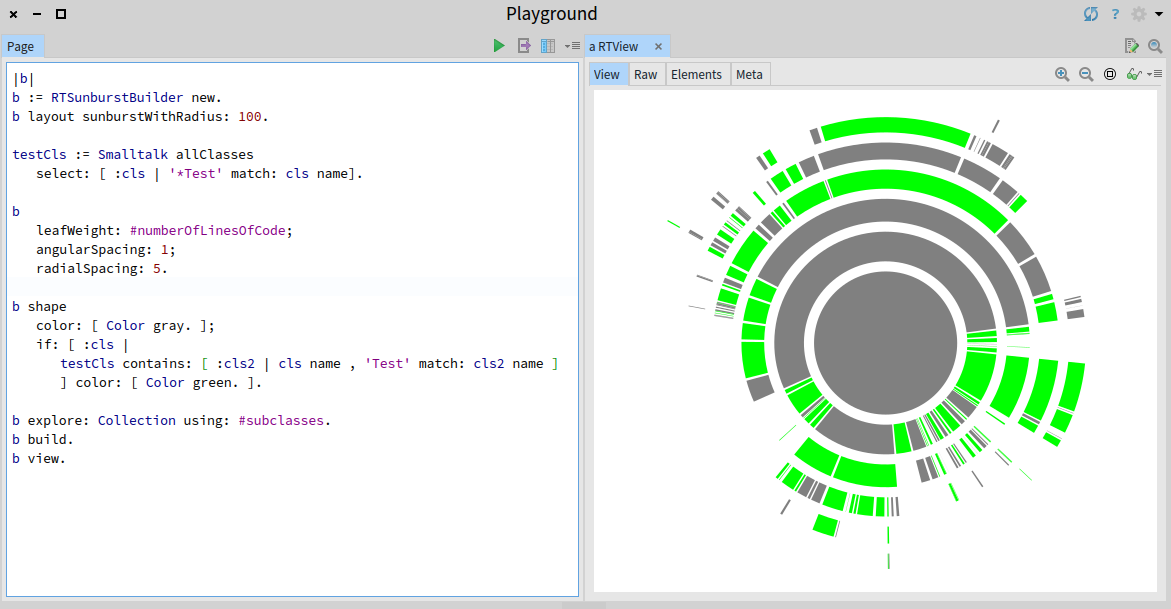
\includegraphics[width=0.9\textwidth]{ex1.png}
  \caption{Output for exercise 1.}
  \label{fig:ex1}
\end{figure}

\section*{Exercise 2}

Here is my code for exercise 2 :

\begin{smalltalkcode}
|b|
b := RTTreeMapBuilder  new.

b shape
  if: [ :obj | obj isClass]
  color: [ :cls |
    (cls subclasses notEmpty) & ('*Array*' match: cls name) 
    ifTrue: [ Color green ]
    ifFalse: [ Color veryLightGray ] ].

b leafWeight: #numberOfLinesOfCode;
  explore: Collection using: #subclasses.
b build.
b view.
\end{smalltalkcode}

Figure \ref{fig:ex2} show the output of the previous listing.

\begin{figure}[h]
  \centering
  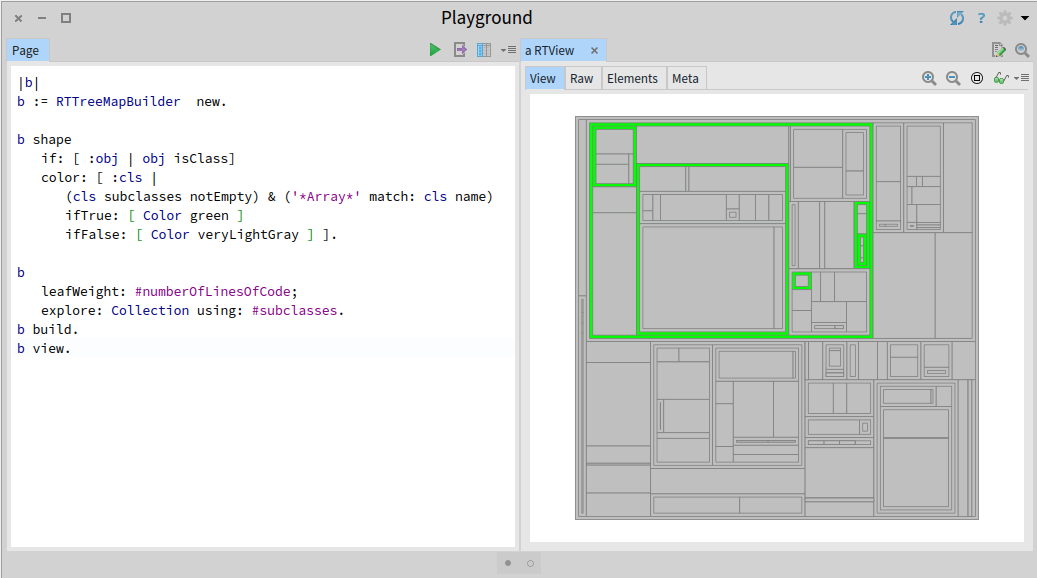
\includegraphics[width=0.9\textwidth]{ex2.png}
  \caption{Output for exercise 2.}
  \label{fig:ex2}
\end{figure}

\newpage

\section*{Exercise 3}

Here is my code for exercise 3 :

\begin{smalltalkcode}
|b|
classes := RTLayout withAllSubclasses , Collection withAllSubclasses.
b := RTMondrian new.
b shape circle
      size: 8;
      color: [ :cls |
        (Collection withAllSubclasses contains: [:cls2 | cls = cls2 ])
          ifTrue: [ Color red ]
          ifFalse: [ Color green ] ].
b nodes: classes.
b edges connectFrom: #superclass.
b shape
  bezierLineFollowing: #superclass;
  color: (Color blue alpha: 0.2).

b normalizer
  normalizeSize: #numberOfMethods using: #sqrt.

b edges
  notUseInLayout;
  connectToAll: #dependentClasses.

b layout cluster.
b build.
b view.
\end{smalltalkcode}

Figure \ref{fig:ex3} show the output of the previous listing.

\begin{figure}[h]
  \centering
  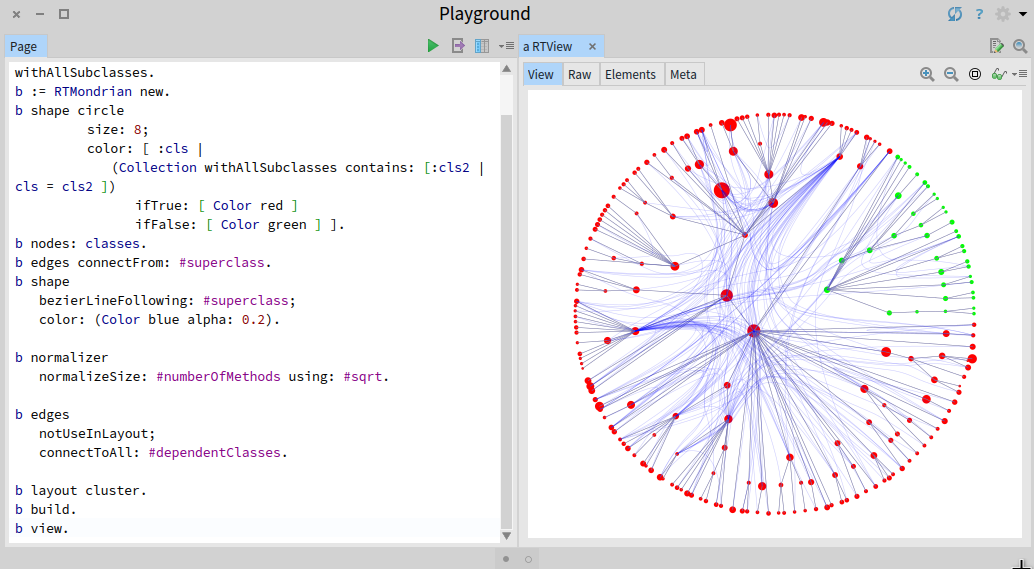
\includegraphics[width=0.9\textwidth]{ex3.png}
  \caption{Output for exercise 3.}
  \label{fig:ex3}
\end{figure}


\section*{Exercise 4}

\subsection*{Sunburst}

\paragraph{Strenghts : }

\begin{itemize}
\item  Great for navigating heirarchical data.
\item  More effective at visualizing a big dataset.
\item  Doesn’t lose the middle layers of hierarchy.
\end{itemize}

\paragraph{Limitations : }

\begin{itemize}
\item Hard to estimate the exact value using arc length.
\item Small, periphery arcs can be hard to see/analyze without interaction.
\end{itemize}

\subsection*{Treemap}

\paragraph{Strenghts : }

\begin{itemize}
\item The eyes visually aggregates rectangles in the same group, allowing to see patterns quickly.
\item Similarity inside a group give relevant information.
\item We can detect anomaly very quickly by seeing a divergent color inside a group.
\end{itemize}

\paragraph{Limitations : }

\begin{itemize}
\item It's hard to show negative and zero value inside a treemap.
\item Printing a treemap is quite hard and label would overlaps very easely.
\end{itemize}

\subsection*{Mondrian}

\paragraph{Strenghts : }

\begin{itemize}
\item We can quickly see dependencies relation and the high dependable class.
\item The interconnection between the subclasses of a specific class.
\item Can handle a large amount of data.
\end{itemize}

\paragraph{Limitations : }

\begin{itemize}
\item We can't easely see precise dependencies if there is too many edges.
\item We can't see dependencies between the leaves of the tree.
\end{itemize}

\end{document}

